% 18 --------------------------------------------------------------------------
% 19 --------------------------------------------------------------------------
\begin{frame}{Application: K-means as an IVF Search Coarse Quantizer}
  \small
  \begin{center}
    \begin{tikzpicture}[node distance=.88cm]
      \node[softbox,text width=3.0cm] (vec) {Database vectors\\$x_i\in\R^d$};
      \node[greenbox,text width=3.0cm,right=of vec] (cent) {K-means centroids\\$\mu_1,\ldots,\mu_K$};
      \node[orangebox,text width=3.0cm,right=of cent] (cell) {Inverted cells\\nearest-center assignment};
      \draw[flow] (vec)--node[above,font=\scriptsize]{train}(cent);
      \draw[flow] (cent)--node[above,font=\scriptsize]{route}(cell);
      \node[softbox,text width=3.0cm,below=1.0cm of cell] (query) {Query vector $q$\\probe $n_{\mathrm{probe}}$ cells};
      \draw[flow] (query)--(cell);
    \end{tikzpicture}
  \end{center}
  \vspace{-.23cm}
  \begin{itemize}\setlength{\itemsep}{.03cm}
    \item $x_i$ is a stored embedding or feature vector; a cluster is one coarse inverted cell.
    \item A query probes selected cells, then exact distances rerank candidates; $n_{\mathrm{probe}}$ trades recall against latency.
  \end{itemize}
\end{frame}

% 20 --------------------------------------------------------------------------
\begin{frame}{Experiments Expose the Preprocessing Assumptions}
  \centering
  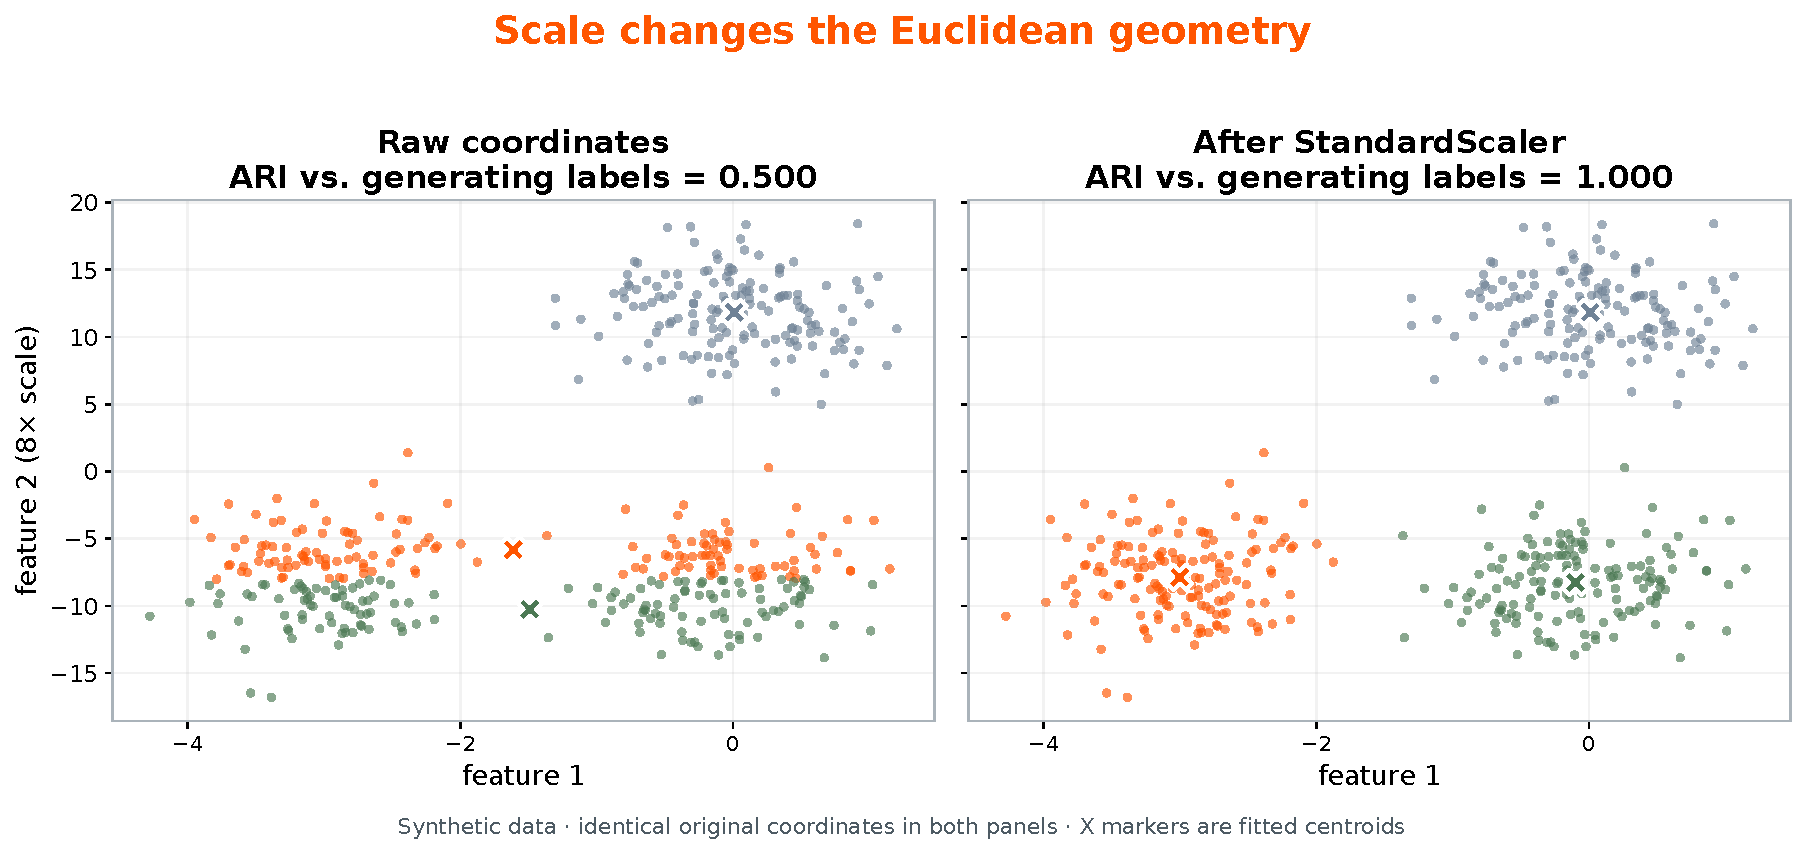
\includegraphics[width=.90\textwidth]{assets/fig_scale.pdf}
\end{frame}

% 21 --------------------------------------------------------------------------
\begin{frame}{Experiments Expose the Geometry Assumptions}
  \centering
  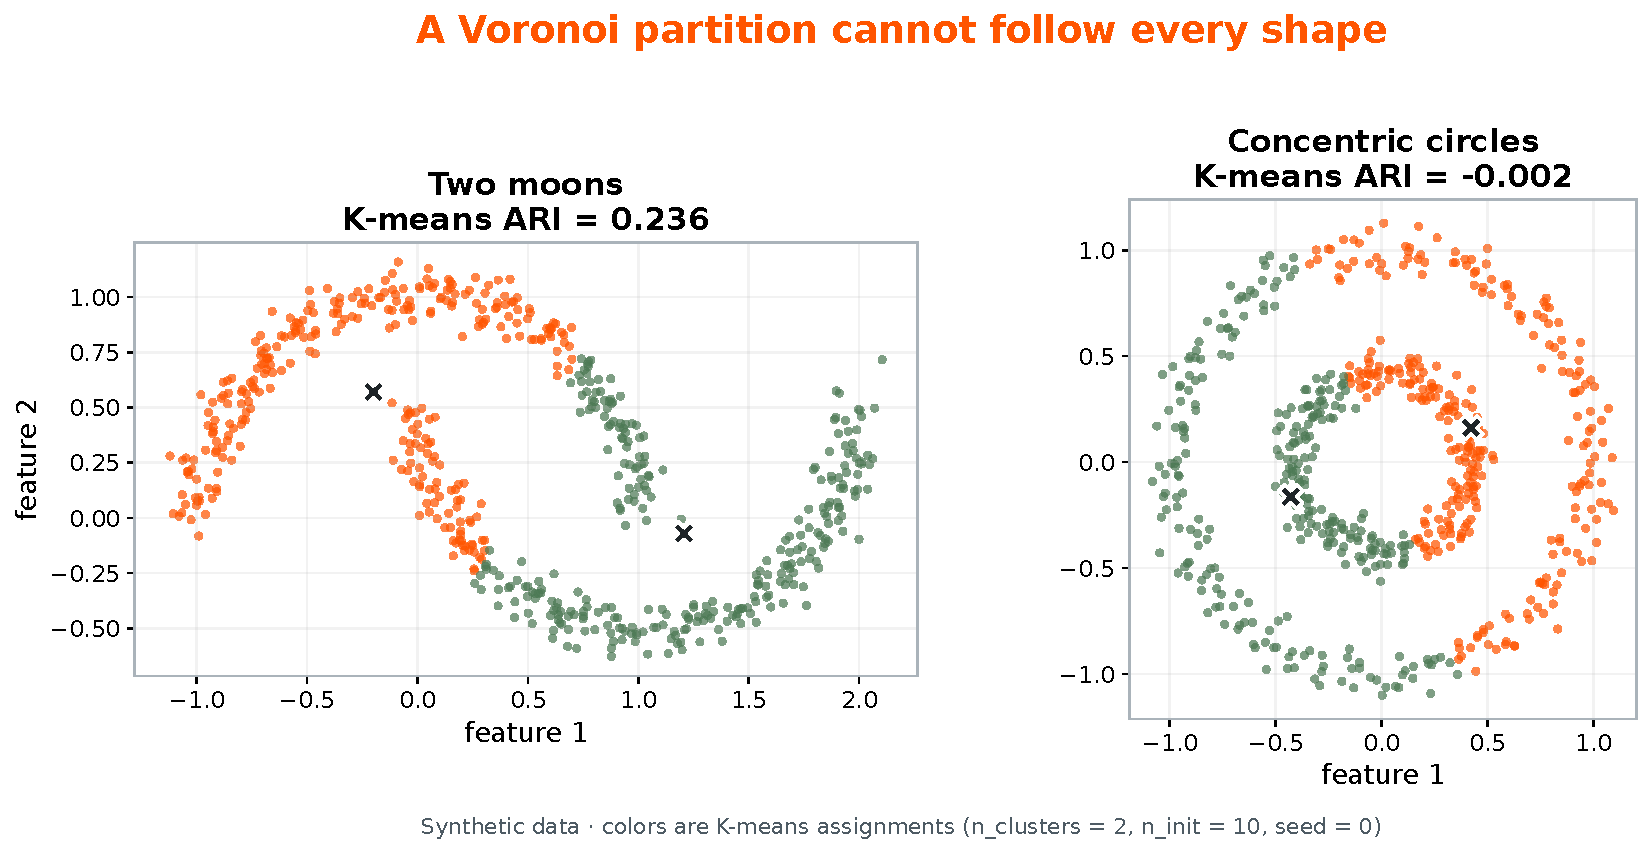
\includegraphics[width=.80\textwidth]{assets/fig_shape_failure.pdf}
\end{frame}

% 22 --------------------------------------------------------------------------
\begin{frame}{Remedies for the Non-regular Case}

      \textbf{Change the representation}
      \begin{itemize}\setlength{\itemsep}{.3cm}
        \item Engineer a radial feature, or use kernel K-means as an implicit nonlinear map.
        \item For concentric rings, $u=x_1^2+x_2^2$ is a radius coordinate.
        \item K-means on $u$ uses a one-dimensional threshold.
      \end{itemize}

  \vspace{.2cm}
  {\scriptsize\color{slideorange}\textbf{Challenge:} standard K-means does not train a feature map; the useful feature must come from data geometry or domain knowledge.}
\end{frame}

% 23 --------------------------------------------------------------------------


% 24 ------------------------------------------------------------------
% 25 --------------------------------------------------------------------------
\begin{frame}{A Practical Reporting Checklist}
  \begin{enumerate}\spaceditems
    \item State what one row $x$ represents and which features were used.
    \item Record scaling, transformations, missing-value handling, and distance.
    \item Run multiple initializations and report objective variability.
    \item Compare several $K$ values using internal and stability diagnostics.
    \item Inspect cluster sizes, profiles, and outliers.
    \item Keep labels or downstream outcomes for validation, not for fitting.
  \end{enumerate}
\end{frame}
